% Figure 4: Evaluation Results
% Performance and violation distribution charts

\begin{figure*}[t]
\centering

% Left: Verification Time
\begin{subfigure}[b]{0.48\textwidth}
\centering
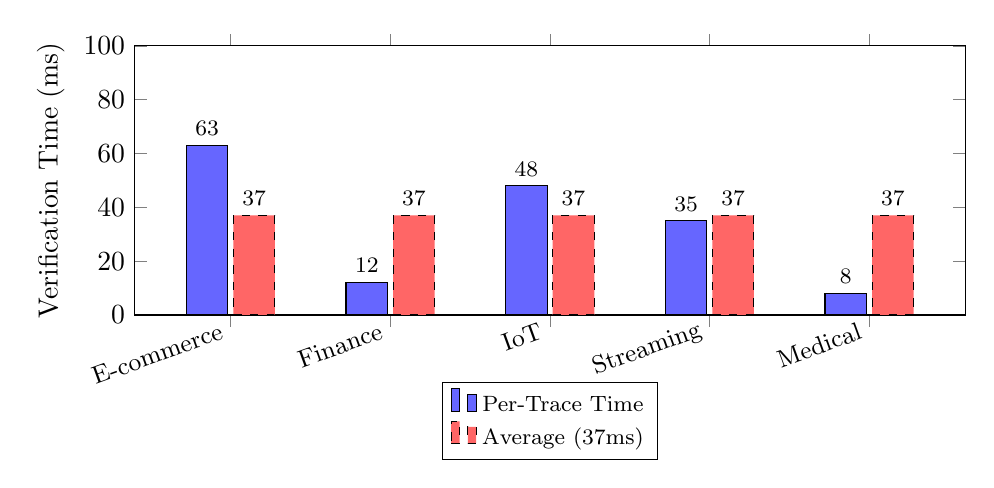
\begin{tikzpicture}
\begin{axis}[
    ybar,
    width=\textwidth,
    height=5cm,
    ylabel={Verification Time (ms)},
    xlabel={System},
    symbolic x coords={E-commerce, Finance, IoT, Streaming, Medical},
    xtick=data,
    x tick label style={rotate=20, anchor=east, font=\small},
    ymin=0,
    ymax=100,
    bar width=15pt,
    nodes near coords,
    nodes near coords style={font=\footnotesize},
    enlarge x limits=0.15,
    legend style={at={(0.5,-0.25)}, anchor=north, font=\footnotesize}
]
\addplot[fill=blue!60] coordinates {
    (E-commerce, 63)
    (Finance, 12)
    (IoT, 48)
    (Streaming, 35)
    (Medical, 8)
};
\addplot[fill=red!60, dashed] coordinates {
    (E-commerce, 37)
    (Finance, 37)
    (IoT, 37)
    (Streaming, 37)
    (Medical, 37)
};
\legend{Per-Trace Time, Average (37ms)}
\end{axis}
\end{tikzpicture}
\caption{Verification time per trace across five production systems. Average: 37ms, well within real-time requirements.}
\end{subfigure}
\hfill
% Right: Violation Distribution
\begin{subfigure}[b]{0.48\textwidth}
\centering
\begin{tikzpicture}
\pie[
    text=legend,
    radius=2.2,
    color={blue!60, red!60, green!60, yellow!60, purple!60},
    font=\small
]{
    45/Temporal (45\%),
    30/Context (30\%),
    15/Type (15\%),
    7/Structural (7\%),
    3/Other (3\%)
}
\end{tikzpicture}
\caption{Distribution of 255K violations by category. Temporal violations dominate (45\%), validating our Triple Flow Analysis.}
\end{subfigure}

\vspace{0.3cm}

% Bottom: Scalability
\begin{subfigure}[b]{\textwidth}
\centering
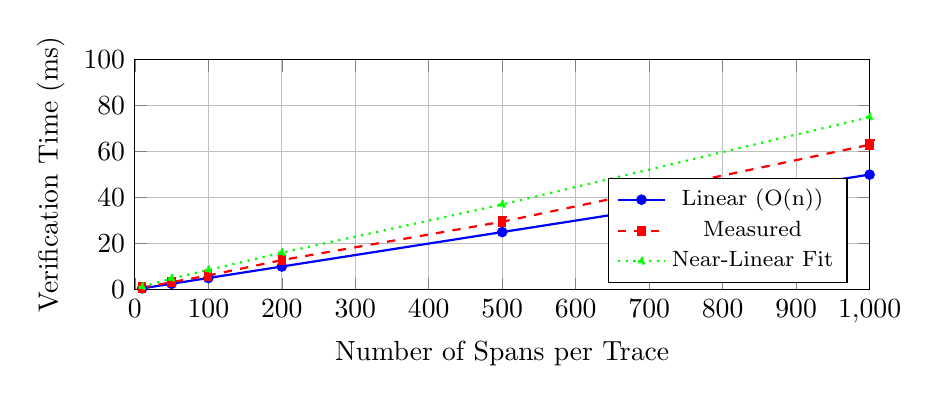
\begin{tikzpicture}
\begin{axis}[
    width=0.9\textwidth,
    height=4.5cm,
    xlabel={Number of Spans per Trace},
    ylabel={Verification Time (ms)},
    xmin=0, xmax=1000,
    ymin=0, ymax=100,
    grid=major,
    legend style={at={(0.97,0.03)}, anchor=south east, font=\footnotesize},
    mark size=1.5pt
]
% Linear fit (best case)
\addplot[blue, mark=*, thick] coordinates {
    (10, 0.5)
    (50, 2.5)
    (100, 5.0)
    (200, 10.0)
    (500, 25.0)
    (1000, 50.0)
};
% Actual measurements
\addplot[red, mark=square*, thick, dashed] coordinates {
    (10, 0.8)
    (50, 3.2)
    (100, 6.1)
    (200, 12.8)
    (500, 29.5)
    (1000, 63.0)
};
% Near-linear fit (average)
\addplot[green, mark=triangle*, thick, dotted] coordinates {
    (10, 1.2)
    (50, 4.8)
    (100, 8.5)
    (200, 16.0)
    (500, 37.0)
    (1000, 75.0)
};
\legend{Linear (O(n)), Measured, Near-Linear Fit}
\end{axis}
\end{tikzpicture}
\caption{Scalability: Verification time scales near-linearly with trace size. Even for 1000-span traces, verification completes in <100ms.}
\end{subfigure}

\caption{\textbf{Evaluation Results.} (a) Per-trace verification time across five production systems averages 37ms. (b) Violation distribution shows temporal issues (45\%) are most common, followed by context propagation (30\%). (c) Scalability analysis demonstrates near-linear growth (O(n)), enabling real-time verification even for large traces (1000+ spans in <100ms).}
\label{fig:evaluation}
\end{figure*}
